In this chapter, we present the step-by-step methodologies, model architectures, and edge deployment pipelines employed in the development of a real-time, high-precision visual inspection system for tallying metallic fasteners on industrial conveyor belts.

The methodology is structured around the following key components:
\begin{enumerate}
    \item \textbf{Dataset Construction and Preprocessing:} Establishing a purpose-built industrial fastener dataset with detailed documentation of data sources, collection methodology, and augmentation strategies.
    \item \textbf{Model Development Strategy:} A two-pronged approach comprising (a) fine-tuning established YOLO variants to establish baseline capabilities, and (b) designing a custom lightweight architecture optimized for edge deployment.
    \item \textbf{Proposed Custom Architecture (YOLOv8-GED):} Design and implementation of the YOLOv8-GED model, integrating novel EMAc2f attention modules, GhostBottleneck efficiency, and DySample dynamic upsampling.
    \item \textbf{Edge Deployment Pipeline:} Optimization and deployment strategies for real-time inference on NVIDIA Jetson platforms.
\end{enumerate}

\begin{figure}[H]
    \centering
    \includegraphics[width=1.0\textwidth]{figures/chapter3/e2e-overview.png}
    \caption{Overview of the methodology for developing a real-time, high-precision fastener counting system on industrial conveyor belts.}
    \label{fig:methodology_overview}
\end{figure}

\section{Dataset Construction and Description}
\label{sec:dataset}

\subsection{Data Collection Context}
During the internship period (July--September 2026), the physical conveyor belt infrastructure was under concurrent development by the mechanical and electrical engineering teams. As a result, actual deployment-domain data from the operational conveyor system was not available during the model development phase. \\

To address this constraint, a \textbf{physical mock-up environment} was constructed in the office setting to simulate the target deployment scenario. This controlled environment enabled systematic data collection under reproducible conditions, allowing for rigorous model development and benchmarking before field deployment.

\subsection{Data Sources and Composition}
The dataset comprises images collected from two primary sources:

\begin{enumerate}
    \item \textbf{Physical Mock-up Collection:} Images captured using a standard industrial camera setup, with metallic fasteners (screws, nuts, and bolts) manually positioned and moved across the camera's field of view to simulate conveyor motion. The collection includes various lighting conditions, object densities, and overlapping configurations.
    
    \item \textbf{Public Datasets:} Supplementary images from publicly available industrial fastener datasets were reviewed for baseline familiarization, including datasets from Roboflow Universe and MVTec (Table~\ref{tab:datasets}).
\end{enumerate}

\begin{table}[htbp]
\centering
\small
\caption{Overview of publicly available fastener datasets reviewed during development.}
\label{tab:datasets}
\begin{tabularx}{\textwidth}{@{}
    >{\raggedright\arraybackslash}X
    >{\raggedright\arraybackslash}X
    >{\centering\arraybackslash}p{0.10\textwidth}
    >{\raggedleft\arraybackslash}p{0.12\textwidth}@{}}
\toprule
\textbf{Dataset} & \textbf{Publisher / Source} & \textbf{Year} & \textbf{Images} \\
\midrule
Bolt Nut Screws \cite{screw-nut-bolt_dataset} & Roboflow Universe & 2026 & 1,500 \\
MVTec Screws \cite{screw-nut-washer-oj52o_dataset} & MVTec Software GmbH & 2023 & 400 \\
Screw and Bolt \cite{screw-and-bolt-nwp0z_dataset} & Roboflow Universe & 2024 &  300\\
\bottomrule
\end{tabularx}
\end{table}

\subsection{Dataset Characteristics}
The collected dataset exhibits the following characteristics:
\begin{itemize}
    \item \textbf{Object Types:} Metallic fasteners including screws, nuts, and bolts (treated as a single class for detection and counting purposes).
    \item \textbf{Image Resolution:} Variable resolutions ranging from 640×480 to 1920×1080 pixels.
    \item \textbf{Object Density:} Images contain varying numbers of objects, from sparse single-object scenes to densely packed configurations with significant occlusion.
    \item \textbf{Background Diversity:} Multiple background types including office surfaces, metallic trays, and simulated conveyor materials.
    \item \textbf{Lighting Conditions:} Natural and artificial lighting variations, including challenging specular highlights on metallic surfaces.
\end{itemize}

Figure~\ref{fig:dataset_samples} presents representative samples from the training dataset, illustrating the diversity of object configurations, lighting conditions, and background variations.

\begin{figure}[htbp]
    \centering
    \begin{subfigure}{0.32\textwidth}
        \centering
        \makebox[\linewidth][c]{\fbox{\includegraphics[width=\linewidth,height=3.2cm,keepaspectratio]{figures/chapter3/datasets/high-res.png}}}
        \caption{Sparse configuration}
    \end{subfigure}
    \hfill
    \begin{subfigure}{0.32\textwidth}
        \centering
        \makebox[\linewidth][c]{\fbox{\includegraphics[width=\linewidth,height=3.2cm,keepaspectratio]{figures/chapter3/datasets/mvtec-sample.png}}}
        \caption{Mixed fastener types}
    \end{subfigure}
    \hfill
    \begin{subfigure}{0.32\textwidth}
        \centering
        \makebox[\linewidth][c]{\fbox{\includegraphics[width=\linewidth,height=3.2cm,keepaspectratio]{figures/chapter3/datasets/noise.png}}}
        \caption{High-density washers}
    \end{subfigure}

    \vspace{0.3cm}
    
    \begin{subfigure}{0.32\textwidth}
        \centering
        \makebox[\linewidth][c]{\fbox{\includegraphics[width=\linewidth,height=3.2cm,keepaspectratio]{figures/chapter3/datasets/diff-position.jpg}}}
        \caption{Varying positions}
    \end{subfigure}
    \hfill
    \begin{subfigure}{0.32\textwidth}
        \centering
        \makebox[\linewidth][c]{\fbox{\includegraphics[width=\linewidth,height=3.2cm,keepaspectratio]{figures/chapter3/datasets/dense.jpg}}}
        \caption{Dense configuration}
    \end{subfigure}
    \hfill
    \begin{subfigure}{0.32\textwidth}
        \centering
        \makebox[\linewidth][c]{\fbox{\includegraphics[width=\linewidth,height=3.2cm,keepaspectratio]{figures/chapter3/datasets/overlapping.jpg}}}
        \caption{Overlapping objects}
    \end{subfigure}
    
    \caption{Representative samples from the training dataset showing diverse fastener types, object densities, spatial arrangements, and challenging scenes with overlapping objects and reflective surfaces.}
    \label{fig:dataset_samples}
\end{figure}

\subsection{Dataset Splitting}

The dataset was partitioned into training, validation, and test sets using a stratified sampling approach to ensure representative distributions of object types, densities, and lighting conditions across all subsets. The final split ratios are detailed in Table \ref{tab:datasets}.

\begin{table}[htbp]
\centering
\caption{Dataset Distribution for Training, Validation, and Testing}
\label{tab:datasets}
% Replaced tabularx with a standard tabular for cleaner numeric alignment
\begin{tabular}{lcc} 
\toprule
\textbf{Dataset Split} & \textbf{Number of Images} & \textbf{Percentage (\%)} \\
\midrule
Training   & 1,824 & 82.91 \\
Validation & 276   & 12.55 \\
Testing    & 100   & 4.55  \\
\midrule
\textbf{Total} & \textbf{2,200} & \textbf{100.00} \\
\bottomrule
\end{tabular}
\end{table}

This splitting strategy ensures that the model is evaluated on unseen data, providing a reliable measure of its generalization capabilities. Specifically, the 276 validation images comprehensively cover fastener characteristics across various lighting conditions and object densities.

Furthermore, while data augmentation techniques are typically employed to balance class distributions and ensure training diversity, the inherent balance and diversity of the collected dataset obviated the need for such methods in this study.

\textbf{Keynote}: Validation set should be done by observation, we cannot just split the dataset randomly, we need to make sure that the validation set is representative of the training set and the test set. We need to make sure that the validation set is not too small or too large, and that it covers all the fasteners characteristics across different lighting conditions and object densities.

\subsection{Preprocessing and Augmentation}
Metallic surfaces present unique challenges for computer vision systems, particularly susceptibility to specular highlights and uneven illumination. To address these challenges, the following preprocessing and augmentation strategies were employed:

\subsubsection{Data Preprocessing}
\textbf{Histogram Equalization (HE)} was applied as a preprocessing step to enhance local contrast and normalize illumination across the dataset.

\subsubsection{Data Augmentation}
During training, comprehensive geometric and photometric augmentations were employed to prevent overfitting and improve model generalization:

\begin{itemize}
    \item \textbf{Mosaic Augmentation ($p=0.5$):} Combines four training images into a single composite image, forcing the network to learn contextual cues from multiple overlapping scenes and improving detection of small, densely packed fasteners.
    
    \item \textbf{MixUp:} Linearly blends pairs of images and their labels to create training samples that encourage linear behavior between classes.
    
    \item \textbf{Random Affine Transformations:}
    \begin{itemize}
        \item Rotation: $\pm 15^\circ$ to simulate varying camera angles
        \item Translation: $\pm 5\%$ of image dimensions
        \item Scaling: $\pm 15\%$ to simulate varying object distances
    \end{itemize}
    
    \item \textbf{HSV Transformations:}
    \begin{itemize}
        \item Hue: $\pm 0.5\%$
        \item Saturation: $\pm 25\%$
        \item Value (Brightness): $\pm 30\%$
    \end{itemize}
    
    \item \textbf{Copy-Paste ($p=0.15$):} Randomly copies and pastes object instances between images to create artificial occlusions and increase object density variations.
\end{itemize}

Mosaic augmentation was disabled for the final 15 epochs (\texttt{close\_mosaic = 15}) to allow the model to converge on unaugmented target distributions.

\begin{figure}[htbp]
    \centering
    
    \begin{subfigure}[b]{0.32\textwidth}
        \centering
        \includegraphics[width=\linewidth,height=3.8cm,keepaspectratio]{figures/chapter3/augmentations/aug_0.jpg}
        \caption{HSV-S Config}
        \label{fig:aug_hsv_s_config}
    \end{subfigure}
    \hfill
    \begin{subfigure}[b]{0.32\textwidth}
        \centering
        \includegraphics[width=\linewidth,height=3.8cm,keepaspectratio]{figures/chapter3/augmentations/aug_8.jpg}
        \caption{HSV-V Config}
        \label{fig:aug_hsv_v_config}
    \end{subfigure}
    \hfill
    \begin{subfigure}[b]{0.32\textwidth}
        \centering
        \includegraphics[width=\linewidth,height=3.8cm,keepaspectratio]{figures/chapter3/augmentations/aug_10.jpg}
        \caption{Low-light screw scene}
        \label{fig:aug_low_light}
    \end{subfigure}
    
    \vspace{1em} 

    \begin{subfigure}[b]{0.32\textwidth}
        \centering
        \includegraphics[width=\linewidth,height=3.8cm,keepaspectratio]{figures/chapter3/augmentations/aug_12.jpg}
        \caption{Grayscale washer scene}
        \label{fig:aug_grayscale_washers}
    \end{subfigure}
    \hfill
    \begin{subfigure}[b]{0.32\textwidth}
        \centering
        \includegraphics[width=\linewidth,height=3.8cm,keepaspectratio]{figures/chapter3/augmentations/aug_14.jpg}
        \caption{Color-shifted screw scene}
        \label{fig:aug_color_shift}
    \end{subfigure}
    \hfill
    \begin{subfigure}[b]{0.32\textwidth}
        \centering
        \includegraphics[width=\linewidth,height=3.8cm,keepaspectratio]{figures/chapter3/augmentations/aug_9.jpg}
        \caption{White-background Scene}
        \label{fig:aug_white_background}
    \end{subfigure}
    
    \caption{Representative samples from the training set after applying the configured geometric and photometric augmentations, including rotation, HSV variation, brightness changes, and grayscale effects.}
    \label{fig:augmentation_samples}
\end{figure}

\section{Model Development Strategy}
\label{sec:model_development}

\begin{figure}[H]
    \includegraphics[width=1.0\textwidth]{figures/chapter3/e2e-overview.png}
    \caption{Full System Flow: From data collection and preprocessing to model development, fine-tuning, and edge deployment on NVIDIA Jetson platforms.}
\end{figure}

The model development follows a two-pronged approach: (1) fine-tuning established YOLO variants to understand baseline performance characteristics and identify architectural limitations, and (2) designing a custom lightweight architecture specifically optimized for the fastener detection task and edge deployment constraints.

The selection of these models was guided by the following considerations:

\begin{itemize}
    \item \textbf{YOLO11s and YOLO11m:} Represent the latest iteration of the YOLO architecture family, offering a balance between accuracy and computational efficiency. The small (s) variant targets edge deployment scenarios, while the medium (m) variant provides higher accuracy at increased computational cost.
    
    \item \textbf{YOLOv26m:} A recent YOLO variant with enhanced feature extraction capabilities, evaluated to assess whether newer architectural improvements benefit the fastener detection domain.
    
    \item \textbf{RT-DETR:} The Real-Time DEtection TRansformer serves as the accuracy ceiling reference. Unlike CNN-based detectors, RT-DETR leverages a transformer encoder-decoder architecture with self-attention mechanisms that capture long-range dependencies, enabling superior handling of occluded objects. Its decoder-based detection head eliminates the need for hand-crafted anchor boxes and Non-Maximum Suppression (NMS) post-processing.
\end{itemize}

\subsubsection{Fine-tuning Protocol}

All models were fine-tuned using transfer learning from pre-trained weights on the COCO dataset. The fine-tuning process followed a standardized protocol:

\begin{enumerate}
    \item \textbf{Weight Initialization:} Models were initialized with pre-trained weights to leverage learned feature representations from large-scale object detection.
    
    \item \textbf{Learning Rate Strategy:} A cosine annealing scheduler with warmup (3 epochs) was employed to ensure stable convergence. The initial learning rate was set to $10^{-3}$ with a final ratio of 0.01.
    
    \item \textbf{Optimization:} The AdamW optimizer was used with weight decay ($5 \times 10^{-4}$) for regularization.
    
    \item \textbf{Training Duration:} Models were trained for 100 epochs with early stopping (patience = 30 epochs) to prevent overfitting.
    
    \item \textbf{Input Resolution:} YOLO variants were trained at $640 \times 640$ pixels (except YOLO11s at $1024 \times 1024$ to assess resolution impact), while RT-DETR was trained at $640 \times 640$ pixels.
\end{enumerate}

\subsubsection{Model Characteristics}

Table~\ref{tab:model_characteristics} summarizes the architectural characteristics and training performance of the fine-tuned models. These metrics establish the baseline capabilities before architectural optimization.

\begin{table}[htbp]
\centering
\caption{Model Characteristics and Training Performance}
\label{tab:model_characteristics}
\begin{tabular}{@{}lccccc@{}}
\toprule
\textbf{Model} & \textbf{Params (M)} & \textbf{FLOPs (G)} & \textbf{mAP@0.5} & \textbf{mAP@0.5:0.95} & \textbf{Imgz} \\ \midrule
YOLO11s        & 9.4  & 21.7  & 0.98 & 0.81 & $1024 \times 1024$ \\
YOLO11m        & 16.4 & 64.1  & 0.981 & 0.817 & $640 \times 640$ \\
YOLOv26m       & 21.7 & 75.0  & 0.98 & 0.81 & $640 \times 640$ \\
RT-DETR (Baseline) & 32 & 110 & 0.985 & 0.82 & $\mathbf{640 \times 640}$ \\ \midrule
\textbf{YOLOv8m-GED} & \textbf{14} & \textbf{55} & \textbf{0.982} & \textbf{0.82} & $\mathbf{640 \times 640}$ \\ \bottomrule
\end{tabular}
\end{table}

\subsubsection{Training Dynamics Visualization}

\begin{figure}[H]
    \label{fig:training_curves}
    \begin{subfigure}{\textwidth}
        \centering
        \fbox{\includegraphics[width=0.8\linewidth]{figures/chapter3/training_args.png}}
        \caption{Training dynamics of fine-tuned models}
    \end{subfigure}
    \hfill
    \begin{subfigure}{\textwidth}
        \centering
        \fbox{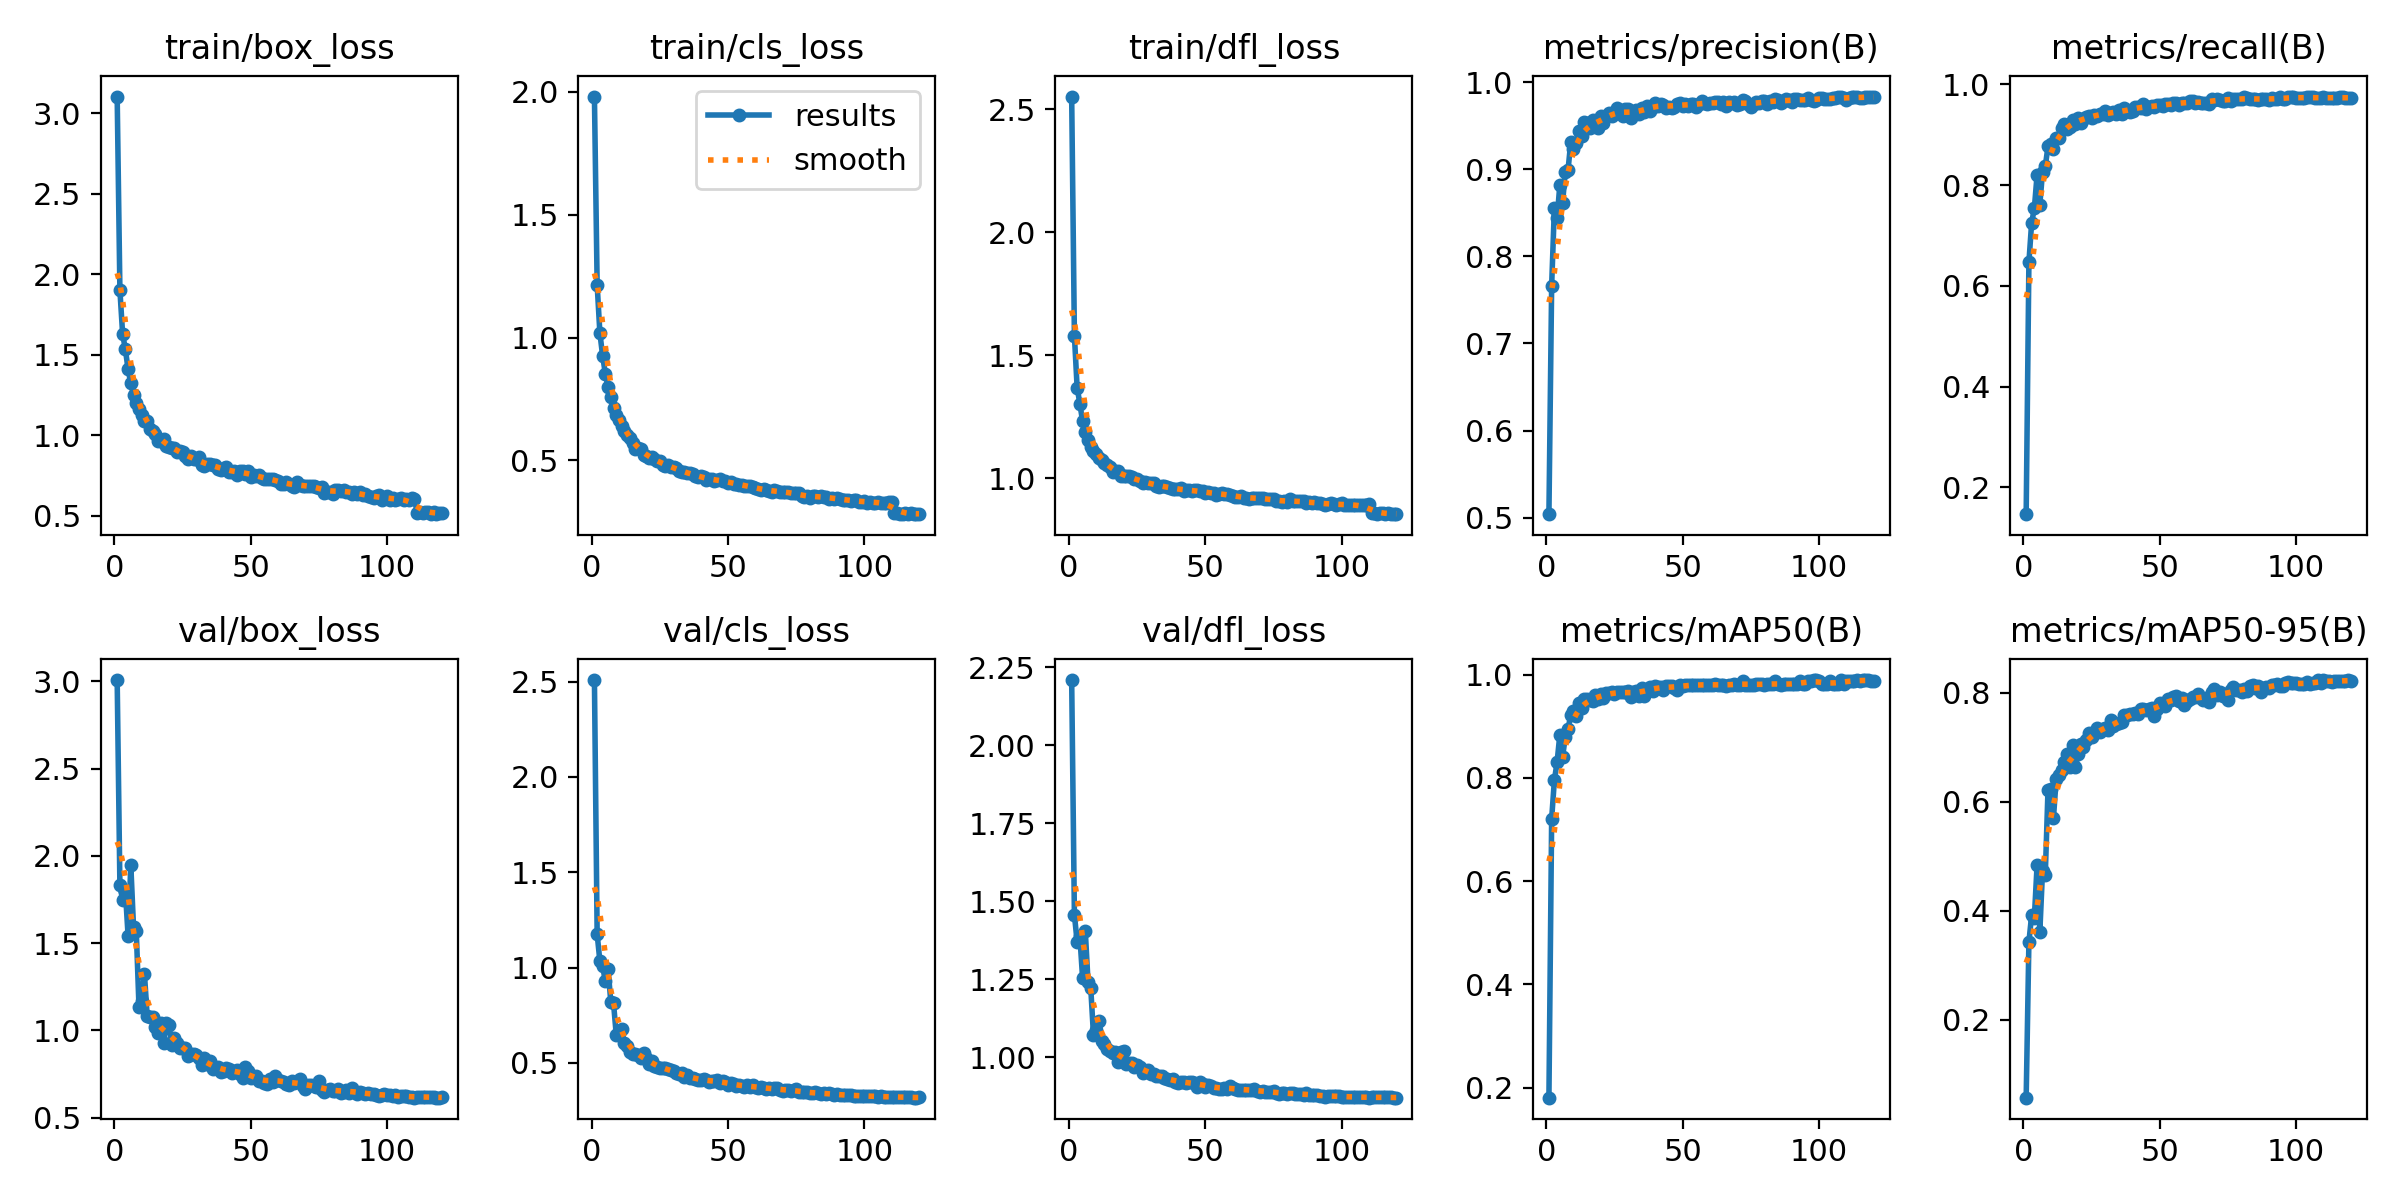
\includegraphics[width=0.8\linewidth]{figures/chapter3/yolov8-ged.png}}
        \caption{Training dynamics performance of YOLOv8-GED (Custom Model)}
    \end{subfigure}
\end{figure}

As we can see, The YOLOv8-GED's (Custom Model) training plot significant better convergence than YOLO Families almost in all categories even with mAP@50 and mAP@95.

\begin{figure}[H]
    \centering
    \begin{subfigure}{0.48\textwidth}
        \centering
        \fbox{\includegraphics[width=0.9\linewidth]{figures/chapter3/val_pred.png}}
        \caption{Validation predictions}
    \end{subfigure}
    \hfill
    \begin{subfigure}{0.48\textwidth}
        \centering
        \fbox{\includegraphics[width=0.9\linewidth]{figures/chapter3/performance.png}}
        \caption{Training Label}
    \end{subfigure}
    \caption{Training validation outputs showing model performance on the fastener dataset.}
    \label{fig:training_validation}
\end{figure}

\subsubsection{Architectural Insights from Fine-tuning}

The fine-tuning process revealed several critical insights that informed the design of the proposed custom architecture:

\begin{enumerate}
    \item \textbf{Small Object Degradation:} Nano-scale and small models exhibited reduced recall for fasteners below critical pixel thresholds, indicating insufficient multi-scale feature preservation in the standard neck architecture.
    
    \item \textbf{Occlusion Sensitivity:} Heavily overlapping fasteners were consistently missed in dense configurations, suggesting that standard convolutions fail to capture the contextual cues needed to infer partially hidden objects.
    
    \item \textbf{Upsampling Artifacts:} Standard nearest-neighbor upsampling in the neck blurred fine-grained metallic textures, leading to false positives on background conveyor reflections.
    
    \item \textbf{Computational Overhead:} While RT-DETR achieved superior accuracy (0.99 mAP@0.5), its high parameter count (32M) and FLOPs (110G) render it impractical for edge deployment on resource-constrained Jetson platforms.
\end{enumerate}

These findings directly motivated the architectural decisions for the proposed YOLOv8-GED model, which aims to maintain high accuracy while significantly reducing computational requirements.

\subsection{Proposed Custom Architecture: YOLOv8-GED}
\label{subsec:proposed_arch}

Building upon the empirical insights from the fine-tuning phase, the \textbf{YOLOv8-GED} architecture was designed as a purpose-built solution for industrial fastener detection. The name reflects its core innovations: \textbf{G}hostBottleneck efficiency, \textbf{E}fficient Multi-scale Attention (EMA), and \textbf{D}ySample dynamic upsampling.

\subsubsection{Design Objectives}

The YOLOv8-GED architecture was designed to address the following objectives:
\begin{itemize}
    \item \textbf{Occlusion Resolution:} Integrate attention mechanisms to capture long-range dependencies and resolve heavily occluded fasteners.
    \item \textbf{Computational Efficiency:} Employ GhostBottleneck to reduce FLOPs while preserving representational capacity.
    \item \textbf{Edge Preservation:} Deploy dynamic upsampling to maintain high-frequency details critical for small, densely packed fasteners.
    \item \textbf{Real-time Throughput:} Achieve $>30$ FPS on NVIDIA Jetson edge platforms through strategic module placement and computational optimization.
\end{itemize}

\subsubsection{Scale Variants}

The architecture is released in three scale configurations, following the Ultralytics depth/width scaling convention (Table~\ref{tab:scales}).

\begin{table}[htbp]
\centering
\caption{YOLOv8-GED scale configurations.}
\label{tab:scales}
\begin{tabular}{lccc}
\toprule
\textbf{Variant} & \textbf{Depth Mult.} & \textbf{Width Mult.} & \textbf{Max Channels} \\ \midrule
YOLOv8-GED-n & 0.50 & 0.25 & 1024 \\
YOLOv8-GED-s & 0.50 & 0.50 & 1024 \\
YOLOv8-GED-m & 0.75 & 0.75 & 768  \\ \bottomrule
\end{tabular}
\end{table}

The medium variant's lower \texttt{max\_channels} cap (768 vs. 1024) intentionally throttles the deepest layers to preserve real-time throughput on the Jetson platform while retaining sufficient representational capacity for the fastener domain.

\subsubsection{Strategic Module Placement}

A key contribution of this work is the \textit{surgical placement} of custom modules. Applying heavy attention mechanisms to shallow layers (P1--P3) yields diminishing returns, as these layers primarily capture low-level edges. Therefore, YOLOv8-GED employs a hybrid backbone strategy:

\begin{itemize}
    \item \textbf{P1--P3 (Shallow):} Retain standard \texttt{Conv} + \texttt{C2f} blocks for efficient, low-level feature extraction.
    
    \item \textbf{P4--P5 (Deep):} Deploy \texttt{EMAc2f} blocks. At these deeper stages, feature maps possess high-level semantic context, making them the optimal location for attention mechanisms to resolve occlusions.
    
    \item \textbf{Neck (P5 $\rightarrow$ P4):} Deploys \texttt{DySample} to prevent semantic blurring during the most critical high-to-medium resolution fusion.
\end{itemize}

\begin{figure}[htbp]
    \centering
    \resizebox{\textwidth}{!}{%
    \begin{tikzpicture}[
        x=1.9cm,
        y=1.15cm,
        >=Latex,
        node distance=0.6cm,
        block/.style={
            rectangle, draw=black!70, line width=0.6pt,
            rounded corners=3pt, text width=2.1cm, align=center,
            minimum height=0.85cm, font=\small\sffamily,
            drop shadow
        },
        conv/.style={block, fill=blue!15},
        c2f/.style={block, fill=green!15},
        emac2f/.style={block, fill=orange!15},
        sppf/.style={block, fill=purple!15},
        dysample/.style={block, fill=red!15},
        upsample/.style={block, fill=cyan!15},
        concat/.style={
            circle, draw=black!70, fill=gray!25,
            minimum size=0.55cm, inner sep=0pt,
            font=\small\sffamily\bfseries, drop shadow
        },
        detect/.style={block, fill=yellow!15, minimum height=1.15cm},
        arrow/.style={
            -{Latex[length=2mm,width=1.5mm]},
            thick, draw=black!80, rounded corners=3pt
        },
        archlabel/.style={font=\scriptsize\sffamily\itshape, text=black!60},
        dim/.style={font=\tiny\sffamily\bfseries, text=black!60},
        grouptitle/.style={
            font=\small\sffamily\bfseries, text=black!80,
            anchor=south, inner sep=0pt
        }
    ]

    \node[conv]    (conv0)    at (0,0)      {Conv \\ 64};
    \node[conv]    (conv1)    at (0,-1.5)   {Conv \\ 128};
    \node[c2f]     (c2f2)     at (0,-3)     {C2f$\times$2 \\ 128};
    \node[conv]    (conv3)    at (0,-4.5)   {Conv \\ 256};
    \node[c2f]     (c2f4)     at (0,-6)     {C2f$\times$2 \\ 256};
    \node[conv]    (conv5)    at (0,-7.5)   {Conv \\ 512};
    \node[emac2f]  (emac2f6)  at (0,-9)     {EMAc2f$\times$3 \\ 512};
    \node[conv]    (conv7)    at (0,-10.5)  {Conv \\ 1024};
    \node[emac2f]  (emac2f8)  at (0,-12)    {EMAc2f$\times$3 \\ 1024};
    \node[sppf]    (sppf9)    at (0,-13.5)  {SPPF \\ 1024};

    \draw[arrow] (conv0)   -- node[right, archlabel] {$s=2$} (conv1);
    \draw[arrow] (conv1)   -- node[right, archlabel] {$s=2$} (c2f2);
    \draw[arrow] (c2f2)    -- node[right, archlabel] {$s=2$} (conv3);
    \draw[arrow] (conv3)   -- node[right, archlabel] {$s=2$} (c2f4);
    \draw[arrow] (c2f4)    -- node[right, archlabel] {$s=2$} (conv5);
    \draw[arrow] (conv5)   -- node[right, archlabel] {$s=2$} (emac2f6);
    \draw[arrow] (emac2f6) -- node[right, archlabel] {$s=2$} (conv7);
    \draw[arrow] (conv7)   -- node[right, archlabel] {$s=2$} (emac2f8);
    \draw[arrow] (emac2f8) -- (sppf9);

    \node[dim, left=0.3cm of c2f4]    (p3) {P3};
    \node[dim, left=0.3cm of emac2f6] (p4) {P4};
    \node[dim, left=0.3cm of sppf9]   (p5) {P5};

    \node[dysample] (dysample10) at (4,-12)   {DySample \\ $\times$2};
    \node[concat]   (concat11)   at (4,-9)    {+};
    \node[emac2f]   (emac2f12)   at (4,-7.5)  {EMAc2f$\times$3 \\ 512};
    \node[upsample] (upsample13) at (4,-6)    {Upsample \\ $\times$2};
    \node[concat]   (concat14)   at (4,-4.5)  {+};
    \node[c2f]      (c2f15)      at (4,-3)    {C2f$\times$3 \\ 256};

    \draw[arrow] (sppf9.east)       -- ++(1.2,0) |- (dysample10.west);
    \draw[arrow] (dysample10.north) -- (concat11.south);
    \draw[arrow] (emac2f6.east)     -- (concat11.west);
    \draw[arrow] (concat11.north)   -- (emac2f12.south);
    \draw[arrow] (emac2f12.north)   -- (upsample13.south);
    \draw[arrow] (upsample13.north) -- (concat14.south);
    \draw[arrow] (c2f4.east)        -- ++(1.2,0) |- (concat14.west);
    \draw[arrow] (concat14.north)   -- (c2f15.south);

    % ---------------- Neck (PAN) ----------------
    \node[conv]   (conv16)   at (8,-3)    {Conv \\ 256};
    \node[concat] (concat17) at (8,-4.5)  {+};
    \node[emac2f] (emac2f18) at (8,-6)    {EMAc2f$\times$3 \\ 512};
    \node[conv]   (conv19)   at (8,-7.5)  {Conv \\ 512};
    \node[concat] (concat20) at (8,-9)    {+};
    \node[emac2f] (emac2f21) at (8,-10.5) {EMAc2f$\times$3 \\ 1024};

    \draw[arrow] (c2f15.east)    -- (conv16.west);
    \draw[arrow] (conv16.south)  -- (concat17.north);
    \draw[arrow] (emac2f12.east) -- ++(1.2,0) |- (concat17.west);
    \draw[arrow] (concat17.south)-- (emac2f18.north);
    \draw[arrow] (emac2f18.south)-- (conv19.north);
    \draw[arrow] (conv19.south)  -- (concat20.north);

    \coordinate (sppf_bottom)   at (0,-14.6);
    \coordinate (pan_left)      at (6.2,-14.6);
    \coordinate (concat20_left) at (6.2,-9);
    \draw[arrow] (sppf9.south) -- (sppf_bottom) -- (pan_left)
                 -- (concat20_left) -- (concat20.west);
    \draw[arrow] (concat20.south) -- (emac2f21.north);

    % ---------------- Head ----------------
    \node[detect] (detect) at (12,-6.75) {Detect \\ $n_c=80$};

    \coordinate (c2f15_top)  at (4,-1.8);
    \coordinate (detect_top) at (12,-1.8);
    \draw[arrow] (c2f15.north) -- (c2f15_top) -- (detect_top) -- (detect.north);

    \draw[arrow] (emac2f18.east) -- ++(1.2,0) |- (detect.west);

    \coordinate (emac21_bottom) at (8,-11.6);
    \coordinate (detect_bottom) at (12,-11.6);
    \draw[arrow] (emac2f21.south) -- (emac21_bottom)
                 -- (detect_bottom) -- (detect.south);

    % ---------------- Background group boxes (NO label=) ----------------
    \begin{scope}[on background layer]
        \node[draw, dashed, rounded corners, fill=gray!5,
              fit=(conv0)(sppf9)(p3)(p4)(p5),
              inner sep=12pt] (backboneBox) {};

        \node[draw, dashed, rounded corners, fill=gray!5,
              fit=(dysample10)(c2f15)(upsample13)(emac2f12)(concat11)(concat14),
              inner sep=12pt] (fpanBox) {};

        \node[draw, dashed, rounded corners, fill=gray!5,
              fit=(conv16)(emac2f21)(concat17)(concat20)(conv19)(emac2f18),
              inner sep=12pt] (panBox) {};

        \node[draw, dashed, rounded corners, fill=gray!5,
              fit=(detect),
              inner sep=15pt] (headBox) {};
    \end{scope}

    % ---------------- Group titles (drawn ABOVE everything) ----------------
    \node[grouptitle] at ([yshift=20pt]backboneBox.north) {Backbone};
    \node[grouptitle] at ([yshift=20pt]fpanBox.north)     {Neck (FPAN)};
    \node[grouptitle] at ([yshift=20pt]panBox.north)      {Neck (PAN)};
    \node[grouptitle] at ([yshift=20pt]headBox.north)     {Head};

    \end{tikzpicture}%
    }
    \caption{Architecture of the proposed YOLOv8-GED model, showing the backbone,
             FPN and PAN necks, EMAc2f blocks, DySample upsampling, and detection head.}
    \label{fig:yolo11ged_arch}
\end{figure}

The cornerstone of YOLOv8-GED is the novel \textbf{EMAc2f} module, designed to replace standard C2f blocks in the deeper stages of the backbone and neck. This module integrates GhostBottleneck efficiency with Efficient Multi-Scale Attention (EMA) to address the occlusion sensitivity identified in the fine-tuning phase.

\paragraph{GhostBottleneck Formulation}

Standard convolutions compute all output feature maps independently, which is computationally redundant. The GhostBottleneck mitigates this by splitting the operation into intrinsic feature generation and cheap linear ``ghost'' feature synthesis. Given an input tensor $X \in \mathbb{R}^{C_{in} \times H \times W}$, the output $Y_{ghost}$ is formulated as:
\begin{equation}
    Y_{intrinsic} = \text{Conv}_{1 \times 1}(X)
\end{equation}
\begin{equation}
    Y_{ghost} = \text{Linear}_{1 \times 1}(\text{DWConv}_{k \times k}(Y_{intrinsic}))
\end{equation}
\begin{equation}
    Y_{out} = \text{Concat}(Y_{intrinsic}, Y_{ghost}) + \text{Shortcut}(X)
\end{equation}
where $\text{DWConv}$ denotes a depthwise convolution. This reduces the computational complexity from $\mathcal{O}(C_{in} C_{out} k^2)$ to $\mathcal{O}(C_{in} C' k^2 + C' C_{out})$, where $C' \approx C_{out}/2$, preserving representational power while halving the FLOPs.

\paragraph{Efficient Multi-Scale Attention (EMA)}

The EMA module is applied as a residual branch to the \texttt{EMAc2f} block. Unlike standard attention that reduces channel dimensions (causing information loss), EMA preserves full channel capacity by operating on grouped features. Let the input be $X \in \mathbb{R}^{B \times C \times H \times W}$, divided into $G$ groups, yielding $X_g \in \mathbb{R}^{(B \cdot G) \times C_g \times H \times W}$.\\

\textbf{Step 1: Cross-Dimensional Spatial Pooling.} To capture long-range spatial dependencies without global flattening, 1D global pooling is applied along the height ($H$) and width ($W$) dimensions:
\begin{equation}
    X_H = \text{Pool}_H(X_g) \in \mathbb{R}^{C_g \times H \times 1}, \quad X_W = \text{Pool}_W(X_g) \in \mathbb{R}^{C_g \times 1 \times W}
\end{equation}
These are concatenated along the spatial dimension and fused via a $1 \times 1$ convolution to model cross-dimensional interactions, then split and passed through a sigmoid activation $\sigma(\cdot)$ to generate directional gating weights $M_H$ and $M_W$.\\

\textbf{Step 2: Dual-Branch Feature Refinement.} The original grouped features are refined through two parallel branches:
\begin{align}
    F_1 &= \text{GroupNorm}\left(X_g \odot \sigma(M_H) \odot \sigma(M_W)\right) \\
    F_2 &= \text{Conv}_{3 \times 3}(X_g)
\end{align}
where $\odot$ denotes the Hadamard (element-wise) product. $F_1$ represents spatially gated features, while $F_2$ captures local neighborhood context.\\

\textbf{Step 3: Channel-Spatial Matrix Aggregation.} To dynamically emphasize fine-grained textures of overlapping metallic fasteners, EMA computes a spatial attention map by multiplying channel-wise importance with spatial feature maps. Let $\text{GAP}(\cdot)$ be Global Average Pooling and $\text{Flat}(\cdot)$ flatten the spatial dimensions to $H \times W$:\\
\begin{align}
    V_1 &= \text{Softmax}(\text{GAP}(F_1)) \in \mathbb{R}^{1 \times C_g} \\
    M_2 &= \text{Flat}(F_2) \in \mathbb{R}^{C_g \times (H \cdot W)} \\
    A_{spatial} &= \sigma\left( \text{Reshape}\Big( V_1 M_2 + V_2 M_1 \Big) \right) \in \mathbb{R}^{1 \times H \times W}
\end{align}
Here, $V_1 M_2$ computes a weighted sum of spatial features in $F_2$ based on the channel importance of $F_1$. The final EMA output is reconstructed to the original batch and channel dimensions:
\begin{equation}
    \text{EMA}(X) = \text{Reshape}_{B, C}\Big( X_g \odot A_{spatial} \Big)
\end{equation}
The final block output is $Y = X_{out} + \text{EMA}(X_{out})$, ensuring stable gradient flow.

\begin{figure}[H]
    \centering
    \fbox{\includegraphics[width=0.9\linewidth]{figures/chapter3/EMAc2f.png}}
    \caption{Attention maps generated by the EMA module demonstrating focus on fastener features, particularly in occluded and densely packed regions.}
    \label{fig:ema}
\end{figure}

\subsubsection{DySample: Dynamic Content-Aware Upsampling}

In the neck's top-down pathway (P5 $\rightarrow$ P4), standard nearest-neighbor or bilinear upsampling blurs high-frequency edges critical for fastener detection, while Deformable Convolutions (DCN) are too computationally heavy. We employ DySample, a lightweight dynamic sampling module.

Given a feature map $X \in \mathbb{R}^{C \times H \times W}$ and an upsampling scale factor $s$, the target resolution is $H' = sH, W' = sW$. The process is defined in three steps:\\

\textbf{1. Offset Prediction:} A lightweight $1 \times 1$ convolution predicts spatial offsets, initialized to zero to ensure the module behaves as standard bilinear upsampling at the start of training:
\begin{equation}
    \Delta P_{raw} = \text{Conv}_{1 \times 1}(X) \in \mathbb{R}^{2s^2 \times H \times W}
\end{equation}

\textbf{2. Grid Generation and Bounding:} The offsets are rearranged via pixel shuffle to match the target resolution, yielding $\Delta P \in \mathbb{R}^{2 \times H' \times W'}$. A normalized base sampling grid $G_{base} \in [-1, 1]^{H' \times W' \times 2}$ is generated. To prevent extreme spatial distortion and ensure training stability, the offsets are bounded using a $\tanh$ activation and scaled by a factor $\lambda$:
\begin{equation}
    G_{dyn} = G_{base} + \tanh(\Delta P) \cdot \lambda, \quad \text{where } \lambda = \frac{2.0}{\max(H, W)}
\end{equation}
The scaling factor $\lambda$ is critical: it converts pixel-level offsets into the normalized $[-1, 1]$ coordinate space required by the grid sampler, preventing gradient explosion.

\textbf{3. Dynamic Bilinear Sampling:} The final upsampled feature map $Y$ is obtained by sampling $X$ at the dynamically perturbed coordinates $G_{\mathrm{dyn}}$:
\begin{equation}
    Y(c, i, j) = \sum_{m,n} X(c, i_m, j_n) \cdot \max(0, 1 - |i - i_m|) \cdot \max(0, 1 - |j - j_n|)
\end{equation}
where $(i_m, j_n)$ are the continuous coordinates derived from $G_{\mathrm{dyn}}(i, j)$. This allows the network to adaptively ``look around'' adjacent pixels based on local content, sharpening upsampled features of small, densely packed fasteners at a fraction of the computational cost of DCN.

\begin{figure}[htbp]
    \centering
    \begin{subfigure}{0.48\linewidth}
        \centering
        \fbox{\includegraphics[width=0.9\linewidth]{figures/chapter3/original.png}}
        \caption{Original feature map}
    \end{subfigure}
    \hfill
    \begin{subfigure}{0.48\linewidth}
        \centering
        \fbox{\includegraphics[width=0.9\linewidth]{figures/chapter3/Dysample.png}}
        \caption{DySample upsampled}
    \end{subfigure}
    \caption{Visual comparison showing how grid offsets in DySample adaptively shift sampling locations to preserve high-frequency details. The DySample upsampled feature map shows sharper edges and better preservation of small fastener features.}
    \label{fig:dysample}
\end{figure}

\begin{figure}[H]
    \centering
    \fbox{\includegraphics[width=0.9\linewidth]{figures/chapter3/ema_dysample.png}}
    \caption{General flow of EMAc2f and DySample}
    \label{fig:ema_flow}
\end{figure}

\section{Training Strategy and Hyperparameters}
\label{sec:training}

All models (RT-DETR, YOLO baselines, and YOLOv8-GED) were trained using PyTorch within the Ultralytics framework. Input images were processed at a spatial resolution of $640 \times 640$ pixels. Optimization was conducted using the AdamW optimizer with an initial learning rate $\eta_0 = 10^{-3}$ and a cosine annealing learning rate scheduler. 

Dynamic data augmentations including Mosaic ($p = 0.5$), HSV transformations, and affine variations were applied during the initial training phase, with Mosaic augmentation disabled for the final 15 epochs (\texttt{close\_mosaic = 15}) to allow convergence on unaugmented target distributions.

The models were trained on Google Colab with a T4 GPU (16GB RAM). The complete training hyperparameters and configuration are summarized in Table~\ref{tab:yolo11_hyperparameters}.

\begin{table}[htbp]
\centering
\small
\caption{Hyperparameter Configuration and Training Setup for YOLO11 Training.}
\label{tab:yolo11_hyperparameters}
\begin{tabularx}{\textwidth}{@{}
    >{\raggedright\arraybackslash}X
    >{\raggedright\arraybackslash}X
    >{\centering\arraybackslash}X
    >{\raggedright\arraybackslash}X@{}}
\toprule
\textbf{Category} & \textbf{Parameter} & \textbf{Value} & \textbf{Description} \\
\midrule
\multicolumn{4}{@{}l}{\textbf{Model \& Data Specifications}} \\
Architecture & \texttt{model} & \texttt{yolo11gedm.yaml} & Custom YOLO11 network layout \\
Dataset Config & \texttt{data} & \texttt{data.yaml} & Path defining data splits and classes \\
Image Resolution & \texttt{imgsz} & $640 \times 640$ & Input image resolution \\
Random Seed & \texttt{seed} & 42 & Fixed seed for reproducibility \\
\midrule
\multicolumn{4}{@{}l}{\textbf{Hardware \& Execution}} \\
Target Device & \texttt{device} & 0 & Single GPU (cuda:0) \\
Mixed Precision & \texttt{amp} & True & FP16 acceleration \\
Data Workers & \texttt{workers} & 2 & Background loading threads \\
Image Caching & \texttt{cache} & True & RAM/Disk caching \\
\midrule
\multicolumn{4}{@{}l}{\textbf{Optimization}} \\
Total Epochs & \texttt{epochs} & 100 & Maximum training epochs \\
Patience & \texttt{patience} & 30 & Early stopping limit \\
Batch Size & \texttt{batch} & 32 & Mini-batch size \\
Optimizer & \texttt{optimizer} & AdamW & Adaptive optimizer \\
Initial LR & \texttt{lr0} & 0.001 & Initial learning rate \\
Final LR Ratio & \texttt{lrf} & 0.01 & Final LR fraction \\
Warmup Epochs & \texttt{warmup\_epochs} & 3.0 & Linear warmup duration \\
Weight Decay & \texttt{weight\_decay} & 0.0005 & $L_2$ regularization \\
LR Scheduler & \texttt{cos\_lr} & True & Cosine annealing \\
\midrule
\multicolumn{4}{@{}l}{\textbf{Augmentations}} \\
HSV-Hue & \texttt{hsv\_h} & 0.005 & Hue adjustment ($\pm 0.5\%$) \\
HSV-Saturation & \texttt{hsv\_s} & 0.25 & Saturation ($\pm 25\%$) \\
HSV-Value & \texttt{hsv\_v} & 0.30 & Brightness ($\pm 30\%$) \\
Rotation & \texttt{degrees} & $15.0^\circ$ & Random rotation range \\
Translation & \texttt{translate} & 0.05 & Random translation ($\pm 5\%$) \\
Scaling & \texttt{scale} & 0.15 & Random scaling ($\pm 15\%$) \\
Mosaic & \texttt{mosaic} & 0.5 & Mosaic blending probability \\
Copy Paste & \texttt{copy\_paste} & 0.15 & Copy-paste probability \\
Close Mosaic & \texttt{close\_mosaic} & 15 & Epochs before deactivation \\
\bottomrule
\end{tabularx}
\end{table}

\subsubsection{Loss Function Formulation}
\label{subsubsec:loss_formulation}

The total objective function optimized during training is a weighted sum of three distinct components:
\begin{equation}
    \mathcal{L}_{total} = \lambda_{box} \mathcal{L}_{box} + \lambda_{obj} \mathcal{L}_{obj} + \lambda_{cls} \mathcal{L}_{cls}
\end{equation}
where $\lambda_{box}$, $\lambda_{obj}$, and $\lambda_{cls}$ are hyperparameters balancing the contribution of each loss term.

\paragraph{Bounding Box Loss ($\mathcal{L}_{box}$)}
To achieve high-precision localization, the bounding box loss combines Complete IoU (CIoU) loss and Distribution Focal Loss (DFL):
\begin{equation}
    \mathcal{L}_{box} = \mathcal{L}_{CIoU} + \mathcal{L}_{DFL}
\end{equation}
The CIoU loss accounts for overlap area, centroid distance, and aspect ratio consistency:
\begin{equation}
    \mathcal{L}_{CIoU} = 1 - \text{IoU} + \frac{\rho^2(b, b^{gt})}{c^2} + \alpha \nu
\end{equation}
where:
\begin{itemize}
    \item $\text{IoU}$ is the Intersection over Union between the predicted box $b$ and ground-truth box $b^{gt}$.
    \item $\rho^2(b, b^{gt})$ is the squared Euclidean distance between the centroids of $b$ and $b^{gt}$.
    \item $c$ is the diagonal length of the smallest enclosing box covering both $b$ and $b^{gt}$.
    \item $\nu$ measures the consistency of the aspect ratio: $\nu = \frac{4}{\pi^2} \left( \arctan\frac{w^{gt}}{h^{gt}} - \arctan\frac{w}{h} \right)^2$.
    \item $\alpha = \frac{\nu}{(1 - \text{IoU}) + \nu}$ is a trade-off parameter.
\end{itemize}

The Distribution Focal Loss (DFL) optimizes the continuous distribution of bounding box boundaries. For a target continuous value $y$ falling between discrete bins $y_i$ and $y_{i+1}$, with predicted softmax probabilities $S_i$ and $S_{i+1}$:
\begin{equation}
    \mathcal{L}_{DFL}(S, y) = -\left( (y_{i+1} - y) \log(S_i) + (y - y_i) \log(S_{i+1}) \right)
\end{equation}
This formulation allows the network to learn ambiguous boundaries (e.g., heavily occluded fasteners) by modeling the boundary location as a probability distribution rather than a single deterministic value.

\paragraph{Objectness Loss ($\mathcal{L}_{obj}$)}
Binary Cross-Entropy (BCE) is used to distinguish fastener objects from the conveyor background. For $N$ anchors, with target $t_i \in \{0, 1\}$ and predicted probability $p_i$:
\begin{equation}
    \mathcal{L}_{obj} = -\frac{1}{N} \sum_{i=1}^{N} \left[ t_i \log(p_i) + (1 - t_i) \log(1 - p_i) \right]
\end{equation}

\paragraph{Classification Loss ($\mathcal{L}_{cls}$)}
Similarly, BCE is applied to multi-class categorization. For $C$ classes, with ground-truth one-hot encoded label $y_{i,c} \in \{0, 1\}$ and predicted probability $p_{i,c}$:
\begin{equation}
    \mathcal{L}_{cls} = -\frac{1}{N} \sum_{i=1}^{N} \sum_{c=1}^{C} \left[ y_{i,c} \log(p_{i,c}) + (1 - y_{i,c}) \log(1 - p_{i,c}) \right]
\end{equation}

\section{Edge Deployment Pipeline}
\label{sec:deployment}

Deploying the trained models onto the NVIDIA Jetson edge platform requires bridging the gap between Python-based training and optimized inference.

\subsection{TensorRT Acceleration}

The PyTorch models are first exported to the Open Neural Network Exchange (ONNX) format. Subsequently, the NVIDIA TensorRT SDK is utilized to optimize the ONNX graph. TensorRT applies layer fusion, kernel auto-tuning, and precision calibration (FP16 or INT8) to maximize throughput on the Jetson's CUDA cores and Tensor cores.

\subsection{Temporal Consistency via ByteTrack}

A critical limitation of frame-wise detection on fast-moving conveyors is prediction oscillation and double-counting due to transient occlusions. To resolve this, the inference pipeline integrates the \textbf{ByteTrack} algorithm.\\

Unlike traditional trackers that discard low-confidence detections, ByteTrack utilizes both high and low-confidence bounding boxes. High-confidence boxes initiate new tracks, while low-confidence boxes are associated with existing tracks based on Intersection over Union (IoU) similarity. This ensures that a fastener temporarily obscured by glare or overlapping parts maintains its unique Track ID, preventing the counting logic from registering it as a new object.

\subsection{Geometric Counting Logic}

Once stabilized Track IDs are established, the Counter module evaluates trajectory centroids against user-defined spatial constraints (Lines, Zones, or Polygons). A fastener is tallied only when its tracked centroid crosses the defined geometric boundary in the correct directional vector, ensuring absolute counting accuracy regardless of conveyor speed or camera angle.

\section{Evaluation Metrics}
\label{sec:metrics}

To comprehensively and objectively evaluate the proposed framework, metrics are strictly divided into accuracy and efficiency categories, defined mathematically as follows:

\subsection{Accuracy Metrics}
\paragraph{Precision and Recall}
Let $TP$ (True Positives) be correctly detected fasteners, $FP$ (False Positives) be background noise or artifacts incorrectly detected as fasteners, and $FN$ (False Negatives) be missed fasteners. Precision ($P$) and Recall ($R$) are defined as:
\begin{equation}
    P = \frac{TP}{TP + FP}, \quad \quad R = \frac{TP}{TP + FN}
\end{equation}

\paragraph{Average Precision (AP)}
AP summarizes the Precision-Recall curve into a single scalar value. It is computed as the area under the Precision-Recall curve $P(R)$:
\begin{equation}
    AP = \int_{0}^{1} P(R) \, dR
\end{equation}
In practice, this is evaluated using the standard 11-point interpolation method or the all-point interpolation method across varying confidence thresholds.

\paragraph{Mean Average Precision (mAP)}
mAP evaluates the overall detection performance across all $C$ object classes. 
\begin{itemize}
    \item \textbf{mAP@0.5:} The mean AP computed at a fixed Intersection over Union (IoU) threshold of $0.50$:
    \begin{equation}
        \text{mAP@0.5} = \frac{1}{C} \sum_{c=1}^{C} AP_c(\text{IoU} = 0.50)
    \end{equation}
    \item \textbf{mAP@0.5:0.95:} The mean AP averaged over multiple IoU thresholds from $0.50$ to $0.95$ with a step size of $0.05$ (i.e., $0.50, 0.55, \dots, 0.95$). This is a stringent metric that heavily penalizes poor localization:
    \begin{equation}
        \text{mAP@0.5:0.95} = \frac{1}{10} \sum_{t=0.50}^{0.95} \left( \frac{1}{C} \sum_{c=1}^{C} AP_c(\text{IoU} = t) \right)
    \end{equation}
\end{itemize}

\subsection{Efficiency and Complexity Metrics}
\paragraph{Inference Latency and Throughput}
Let $T_{inference}$ be the average time required to process a single frame on the target NVIDIA Jetson hardware, excluding I/O and pre/post-processing overhead. The throughput is defined as:
\begin{equation}
    \text{FPS} = \frac{1}{T_{inference}}
\end{equation}
where FPS denotes Frames Per Second. Real-time performance is strictly defined as $\text{FPS} \geq 30$.

\paragraph{Model Complexity}
The computational footprint is quantified by two rigorous measures:
\begin{itemize}
    \item \textbf{Parameter Count ($N_{params}$):} The total number of trainable weights and biases in the network, measured in Millions (M). This directly correlates with model memory footprint.
    \item \textbf{Floating Point Operations (FLOPs):} The total number of multiply-accumulate (MAC) operations required for a single forward pass of an input of resolution $H \times W$, measured in Billions (G). For a standard convolution layer, this is calculated as:
    \begin{equation}
        \text{FLOPs} \approx 2 \cdot H \cdot W \cdot C_{in} \cdot C_{out} \cdot K_h \cdot K_w
    \end{equation}
    where $C_{in}$ and $C_{out}$ are input and output channels, and $K_h, K_w$ are kernel dimensions. This metric strictly bounds the theoretical computational demand on the edge device.
\end{itemize}

\section{Summary}
\label{sec:chapter3_summary}

This chapter detailed the systematic methodology behind the development of the fastener detection framework. Beginning with the construction of a purpose-built dataset under physical mock-up conditions, we established comprehensive preprocessing and augmentation strategies tailored to metallic object detection.\\

The model development followed a two-pronged approach: (1) fine-tuning established YOLO variants (YOLO11s, YOLO11m, YOLOv26m) and RT-DETR to understand baseline capabilities and identify architectural limitations, and (2) designing the YOLOv8-GED architecture as a purpose-built solution. The YOLOv8-GED model strategically integrates EMAc2f attention modules for occlusion resolution, GhostBottleneck for computational efficiency, and DySample for edge-preserving upsampling.\\

The integration of these custom modules into a hybrid backbone, combined with ByteTrack for temporal stability and TensorRT for edge acceleration, forms a complete, highly optimized pipeline for industrial fastener tallying. The following chapter will present the quantitative benchmarking results, ablation studies, and real-world validation of these architectural choices on the target edge hardware.

